\documentclass{report}
\usepackage{amsmath, nccmath}
\usepackage{float}
\usepackage{graphicx}
\usepackage{svg}
\graphicspath{ {./figures/} }
\begin{document}

\chapter{Clustering Methods}

\section{Two-step Method}
The two-step method was originally devised by Katya Kosheleva in 2012 to model the evolution of yeast populations, and has since been modified to accomodate a wider array of experimental designs. Since each frequency measurement is analagous to the probability of a mutation being detected at a given timepoint, we can use the binomial distribution to test whether two sets of frequency measurements represent the same underlying series. There are a few key assumptions that must be made:

\begin{enumerate}
\item The separation between two mutational trajectories that belong to the same genotype is due to measurement error and the error is normally distributed.
\item Each sampled timepoint over the course of an evolutionary experiment is perfectly representative of the population as a whole. That is, mutations that first appear at large frequencies (i.e. 60\%) must have appeared and risen to that level since the most resently sampled timepoint (i.e. it was not simply missed during the sampling step).
\item Any two mutational trajectories will have at least one common timepoint where both are detected and not fixed.
\end{enumerate}

Assumption 3 is particularly troublesum, since there are typically a few mutational trajectories which do not satisfy this assumption, and these cases must be handled differently (described after the calculation method).
The two-step method also requires the user to specify a couple variables:

\begin{description}
\item[similarity cutoff] \verb|--similarity-cutoff 0.05| Used during the agglomerative clustering step for both methods to group trajectories into initial genotypes.
\item[link cutoff] \verb|--link-cutoff 0.25| Used during the unlinking step to determine if a genotype contains at least one pair of mutational 
  trajectories that do not belong to the same genotype.
  \textbf{Note: This is only used if the two-step clustering method is being used.}
\end{description}

The two-step method essentially tests whether the average distance between two series is statistically significant given the uncertainty in the data. If the difference is not statistically significant, the two genotypes are grouped into the same genotype. This is done for all possible pairs of mutational trajectories in the dataset.

\subsection{Agglomerative clustering based on similarity}

The two-step method defines each mutational frequency as the probability of a mutation being detected given $n$ independent measurements. This is best characterized by the binomial distribution which models the probability of a "success" (in this case, the presence of a specific mutation) given the probability of success (the measured frequency).

\subsection{Similarity Calculation}

If there are two series $X$ and $Y$ that represent a pair of mutational trajectories with $n$ timepoints such that $X=\{X_0,X_1,...,X_n\}$
and $Y=\{Y_0,Y_1,...,Y_n\}$ where $f_{detected} < X_i,Y_i < f_{fixed}$, there exists a series $\mu$ representing the mean probability of success
(a mutation is present) at any time point $i$ such that $\mu=\{\mu_0,\mu_1,...,\mu_n\}$, where $\mu_i=\frac{X_i+Y_i}{2}$ for $0\le i \le n$.

Since $\mu$ represents the set of average frequencies (corresponding to the average probability of success) between the two series at each timepoint and the variance of a binomial distribution as a whole is defined as $\sigma^2=np(1-p)$, the variance $\sigma_i^2$ for each element $\mu_i \in \mu$ is $\sigma_i^2=\mu_i(1-\mu_i)$ for an individual element $\mu_i$.

The variance of the series as a whole is then
\begin{equation}
\sigma^2 = \frac{1}{n^2}\sum_{i=0}^n \sigma_i^2=\frac{1}{n^2}\sum_{i=0}^n \mu_i(1-\mu_i),
\mu_i=\frac{X_i+Y_i}{2}
\end{equation}

Since we are interested in whether the difference between the two series $X$ and $Y$ is statistically significant, we define the difference series $d$ such that $d={d_0,d_1,...,d_n}$ and $d_i=|X_i-Y_i|$. We can then check whether the mean difference in probabilities $\bar{d}$ is
statistically significant using the error function.

The error function has the following interpretation: for a normally-distributed random variable $X \ge 0$, $erf(x)$ gives the probability of $X$ falling in the range $[-x,x]$.

The error function is related to the cumulative distribution function of the normal distribution (denoted as $\Phi$) by
\begin{equation}
F(x|\mu,\sigma) = \Phi\bigg(\frac{x-\mu}{\sigma}\bigg)= \frac{1}{2}\bigg[1 + erf \bigg(\frac{x-\mu}{\sqrt{2\sigma^2}}\bigg)\bigg]
\end{equation}

We want to calculate the probability that the average difference $\bar{d}$ between the two mutational trajectories exceeds the amount expected given the uncertainty in our data:
\[
P(\bar{d} > x) = 1-F(\bar{d}|\mu, \sigma) = \frac{1}{2} - \frac{1}{2}erf \bigg(\frac{\bar{d}}{\sqrt{2\sigma^2}}\bigg)
\]
\begin{equation}
P(\bar{d}<-x, x < \bar{d}) = 1 - erf \bigg(\frac{\bar{d}}{\sqrt{2\sigma^2}}\bigg)
\end{equation}

However, as noted above, this test is only performed for the measurements in $X$ and $Y$ which satisfy the requirement $f_{detected} < f <f_{fixed}$ for $f \in X,Y$. timepoints where neither series satisfy this requirement are discarded. If there is no overlap between the timepoints in $X$ and $Y$ after these timepoints have been discarded then the above probability calculation cannot be done. This does not mean that both series are unrelated; if both timepoints fix immediately (at the timepoint they are first detected) during the same timepoint, they should be added to the same genotype. There is an additional test to address this edge case. If two trajectories are fixed at 3 or more common timepoints they are assigned to the same genotype.
\begin{figure}[h]
  \caption{Values of $p$ vs. $\bar{d}$ for various values of $\sigma^2$. Note that as the variance increases, the average distance between series is allowed to grow larger before the series are considered separate genotypes ($p$=0.05, red line).}
  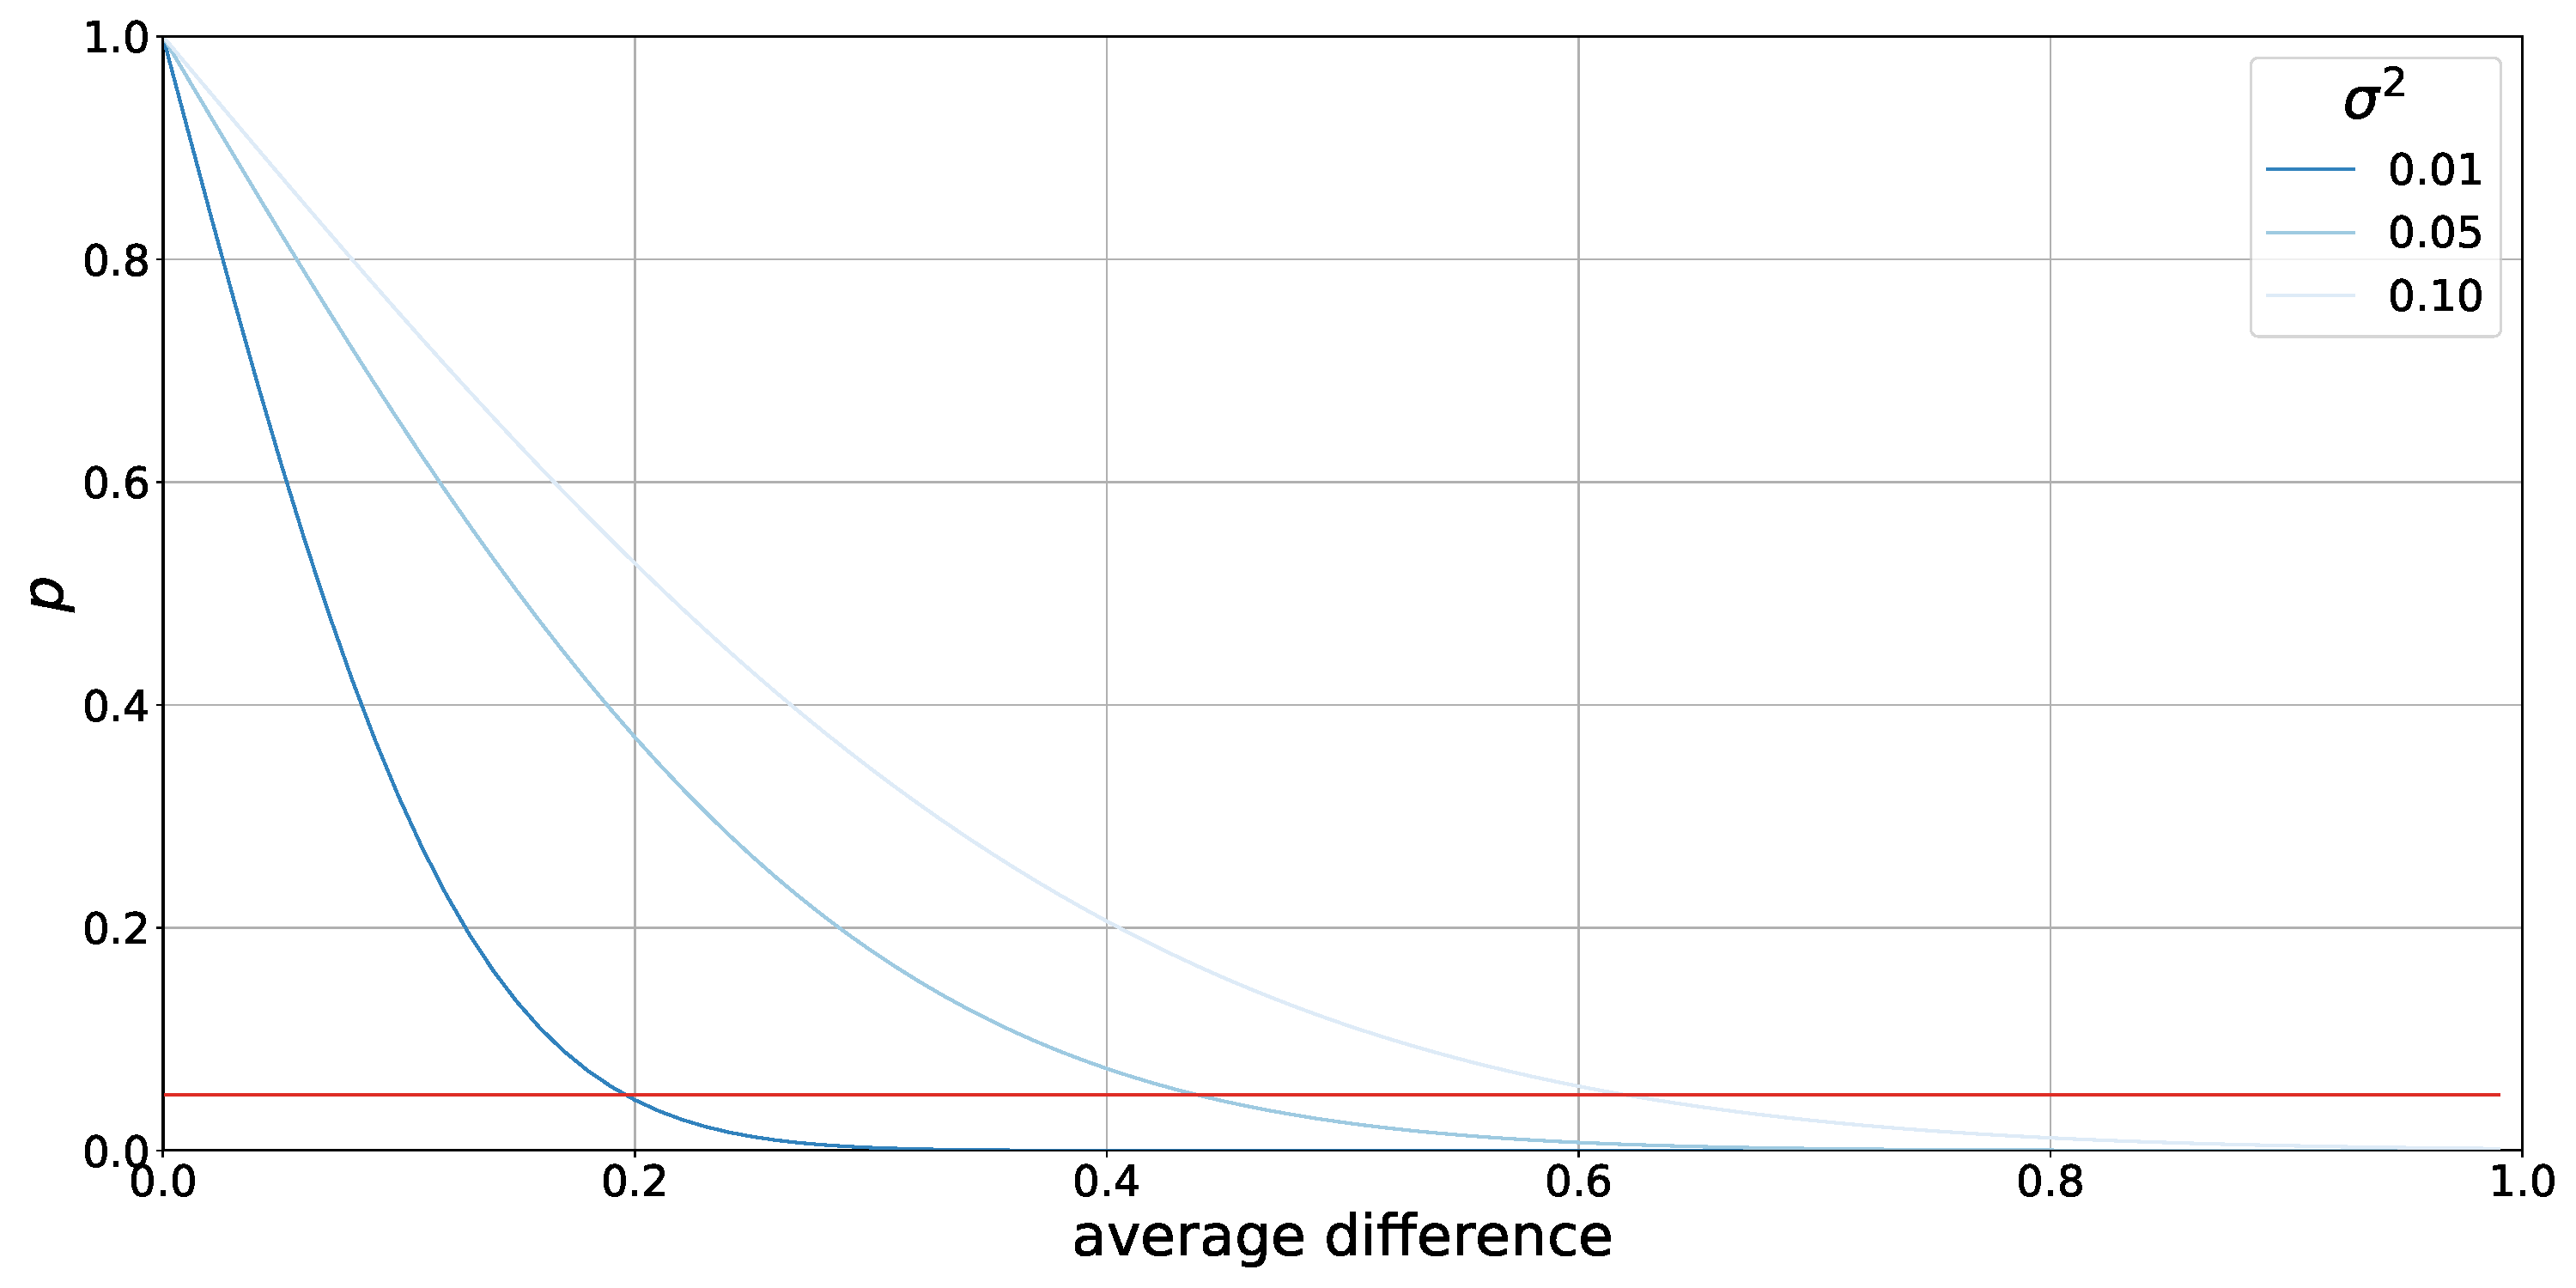
\includegraphics[width=\linewidth]{binomial_probability.pdf}
\end{figure}

Given two mutational series from the same genotype:

\begin{table}[H]
  \begin{center}
    \begin{tabular}{l|llllll}
    Trajectory & 0 & 1 & 2 & 3 & 4 & 5 \\
    \hline
    trajectory-A1 & 0 & 0 & 0 & 0.100 & 0.500 & 0.500 \\
    trajectory-A2 & 0 & 0 & 0 & 0.060 & 0.060 & 0.350 \\
    \end{tabular}
  \end{center}
\end{table}

Calculate the series for $\mu$, $\sigma^2$, and $d$:

\begin{table}[H]
  \begin{center}
    \begin{tabular}{l|llllll}
    symbol & 0 & 1 & 2 & 3 & 4 & 5 \\
    \hline
    $\mu_i$         & 0 & 0 & 0 & 0.080 & 0.425 & 0.450 \\
    $\sigma_i^2$    & 0 & 0 & 0 & 0.221 & 0.733 & 0.743 \\
    $d_i$           & 0 & 0 & 0 & 0.040 & 0.150 & 0.100 \\
    \end{tabular}
  \end{center}
\end{table}

The computation for the variance and average difference for the paired series is relatively straightforward:

\begin{align*}
  \sigma^2 &= (0.074+0.244+0.248)/9=0.062 \\
  \bar{d}  &= (0.040+0.150+0.100)/3=0.097 \\
\end{align*}

Once $\sigma^2$ and $\bar{d}$ are known we can use the error function to calculate the p-value corresponding to the probability that $\bar{d}$ exceeds out upper and lower bounds:

\[
p = 1 - erf \bigg(\frac{\bar{d}}{\sqrt{2\sigma^2}}\bigg)=
1-erf \bigg(\frac{0.097}{\sqrt{2 \times 0.062}}\bigg)=
1-erf(0.091)=1-0.300=0.700
\]

Note that while these values were rounded to three decimal places for brevity, the actual calculation used the raw numbers from each calculation.

\subsubsection{Example}

Given these two mutational trajectories, should the genotypes they belong to be merged?

\begin{table}[H]
  \begin{center}
    \begin{tabular}{l|llllll}
      Trajectory & 0 & 1 & 2 & 3 & 4 & 5 \\
    \hline
     trajectory-A1 & 0 & 0     & 0     & 0.100 & 0.500 & 0.500 \\
     trajectory-B1 & 0 & 0.070 & 0.100 & 0.020 & 0.010 & 0   \\
    \end{tabular}
  \end{center}
\end{table}

Calculate the series for $\mu$, $\sigma^2$, and $d$:

\begin{table}[H]
  \begin{center}
    \begin{tabular}{l|llllll}
      & 0 & 1 & 2 & 3 & 4 & 5 \\
    \hline
     mu         & 0 & 0.035  & 0.050 & 0.060 & 0.255 & 0.250 \\
     sigma      & 0 & 0.034  & 0.048 & 0.056 & 0.190 & 0.188 \\
     d          & 0 & 0.070  & 0.100 & 0.080 & 0.490 & 0.500 \\
    \end{tabular}
  \end{center}
\end{table}

The computation for the variance and average difference for the paired series is relatively straightforward:

\begin{align*}
\sigma^2 &= (0.034+0.048+0.056+0.190+0.189)/16=0.021 \\
\bar{d}  &= \frac{1}{5}(0.07+0.1+0.08+0.49+0.5)=0.248 \\
\end{align*}
\[
p = 1 - erf \bigg(\frac{\bar{d}}{\sqrt{2\sigma^2}}\bigg)=
1-erf \bigg(\frac{0.248}{\sqrt{2 \times 0.021}}\bigg)=
1-erf(1.223)=1-0.916=0.084
\]


\subsection{Unlinking based on maximal distance}

An important note about the above clustering method is that a pair of mutations is added to a genotype if the similarity of only one of the trajectories A in a given pair of trajectories A and B is sufficiently similar to the root trajectory G that forms the genotype. While trajectory B may be sufficiently similar to trajectory A, and trajectory A is sufficiently similar to trajectory G, trajectory B may not be similar enough to trajectory G to warrant its inclusion into the genotype. Due to this, each genotype must be split into child genotypes each of which *is* sufficiently similar.

For each genotype with at least one pair of trajectories that have a p-value less than $link_cutoff$ (defined above),
the two trajectories with the least similarity between them (as determined by the above test of probability) are extracted and form two new genotypes.
All remaining trajectories in the original genotype are then sorted into one of these new genotypes based on which of the root trajectories of each genotype is
most similar. This process continues until no new genotypes are created.

\subsubsection{Example}

For the three mutational trajectories in the above examples, the pairwise p-values are:
\begin{table}[H]
  \begin{center}
  \begin{tabular}{l|ll}
    $p$ & A2 & B1 \\
    \hline
    A1 & 0.700 & 0.084 \\
    A2 &       & 0.177 \\
  \end{tabular}
\end{center}
\end{table}

The two genotypes with the least similarity are A1 and B1. Since at least one pair of trajectories in this genotype have a p-value less than the default \textbf{linkcutoff} value of 0.25, these two trajectories are split into their own genotypes, and the remaining trajectories (in this case, A2) are sorted into the genotype that is most similar. The resulting genotypes are then:

\begin{table}[H]
  \begin{center}
    \begin{tabular}{c|c}
    Genotype A & Genotype B \\
    \hline
    trajectory-A1 & trajectory-B1 \\
    trajectory-A2 &  \\
    \end{tabular}
  \end{center}
\end{table}

\subsection{Hierarchical Method}
The second clustering method implemented relied on hierarchical clustering based on a specified distance metric (a measurement of the similarity of two series). 
It was implemented in an attempt to address the assumptions made by the two step method.

Hierarchical clustering attempts to group elements together based on a measure of similarity. 
Each mutational trajectory is first assigned to its own cluster, 
then clusters are progressively combined based on a specified similarity metric until the maximum distance between any two points in a cluster exceeds a given breakpoint. 
Hierarchical clustering does not require a pre-defined number of clusters (compared to k-means clustering) 
which is advantageous since the resulting number of genotypes is unknown.

\subsubsection{Distance metrics}
There are currently 3 distance metrics implemented in the scripts: binomial distance (described above), pearson's distance, and minkowski's distance. 
Each is designed to measure the similarity of two series but do so by measuring different features.


\subsubsection{Pearson's distance}
Pearson's distance (based on Pearson's correlation coefficient) measures the similarity of two series based on how well they correlate. 
It essentially checks whether a proportional increase seen in one series is also seen in the other. 
It is best used when there are a large number of measurements available in both series, but can be adjusted (see below) to work with small datasets.

Pearson's correlation coefficient is a measure of the linear correlation between two series.
It has a value between -1 and 1 which can be interpreted as such:
\begin{enumerate}
  \item A value of 1 indicates perfect correlation between two series
  \item A value of 0 indicates there is no correlation between two series
  \item A value of -1 indicates perfect negative correlation between two series.
\end{enumerate}

Pearsons's correlation coefficient can be calculated as

\begin{equation}
r(X,Y) = \frac{cov(X,Y)}{\sigma_X \sigma_Y} =
\frac{\sum_{i=0}^n (X_i-\bar{X})(Y_i-\bar{Y})}{\sigma_X \sigma_Y}
\end{equation}

Since distance values between two series cannot be negative, Pearsons's distance metric is simply $1-r(X,Y)$. Unfortunately, since the number of sampled timepoints in a typical evolutionary experiment is relatively low, the sample coefficient derived from $r(X,Y)$ is not an unbiased estimate for the population coefficient. After adjusting for this, the resulting estimate of the pearson correlation coefficient for the sample set is

\begin{equation}
r_{adjusted}(X,Y) = \sqrt{1-\frac{(1-r^2)(n-1)}{n-2}}
\end{equation}

which approches the population coefficient for large values of $n$.


\subsubsection{Minkowski distance}
The minkowski distance measures the similarity of any two series based on the distance between the two trajectories at every sampled timepoint.

The generalized minkowski distance between two series $X$ and $Y$ is defined as
\begin{equation}
d_m=\bigg[\sum_{i=0}^n|X_i-Y_i|^p\bigg]^\frac{1}{p}, p \ge 1
\end{equation}

where $p=2$ (equivilent to the euclidean distance) for these scripts.

\subsubsection{Nearest-neighbor Clustering}

Once the distance between all possible pairs of mutational trajectories has been calculated, 
each trajectory can be grouped with other trajectories that are sufficiently similar. 
Trajectories are first assigned to their own cluster, 
then clusters are merged with similar clusters until the mean distance between trajectories in the cluster exceeds the quantile of all no-zero distances
specified by the similarity cutoff.

\subsubsection{Default Clustering Methods}

The scripts currently use the hierarchical method by default.
The two-step method and the desired distance metric can be selected using the `--method` and `--metric` options, respectively.

\subsection{Comparison of Clustering Methods}

For the B1 testing population, the two-step method produces the following clusters:
\begin{figure}
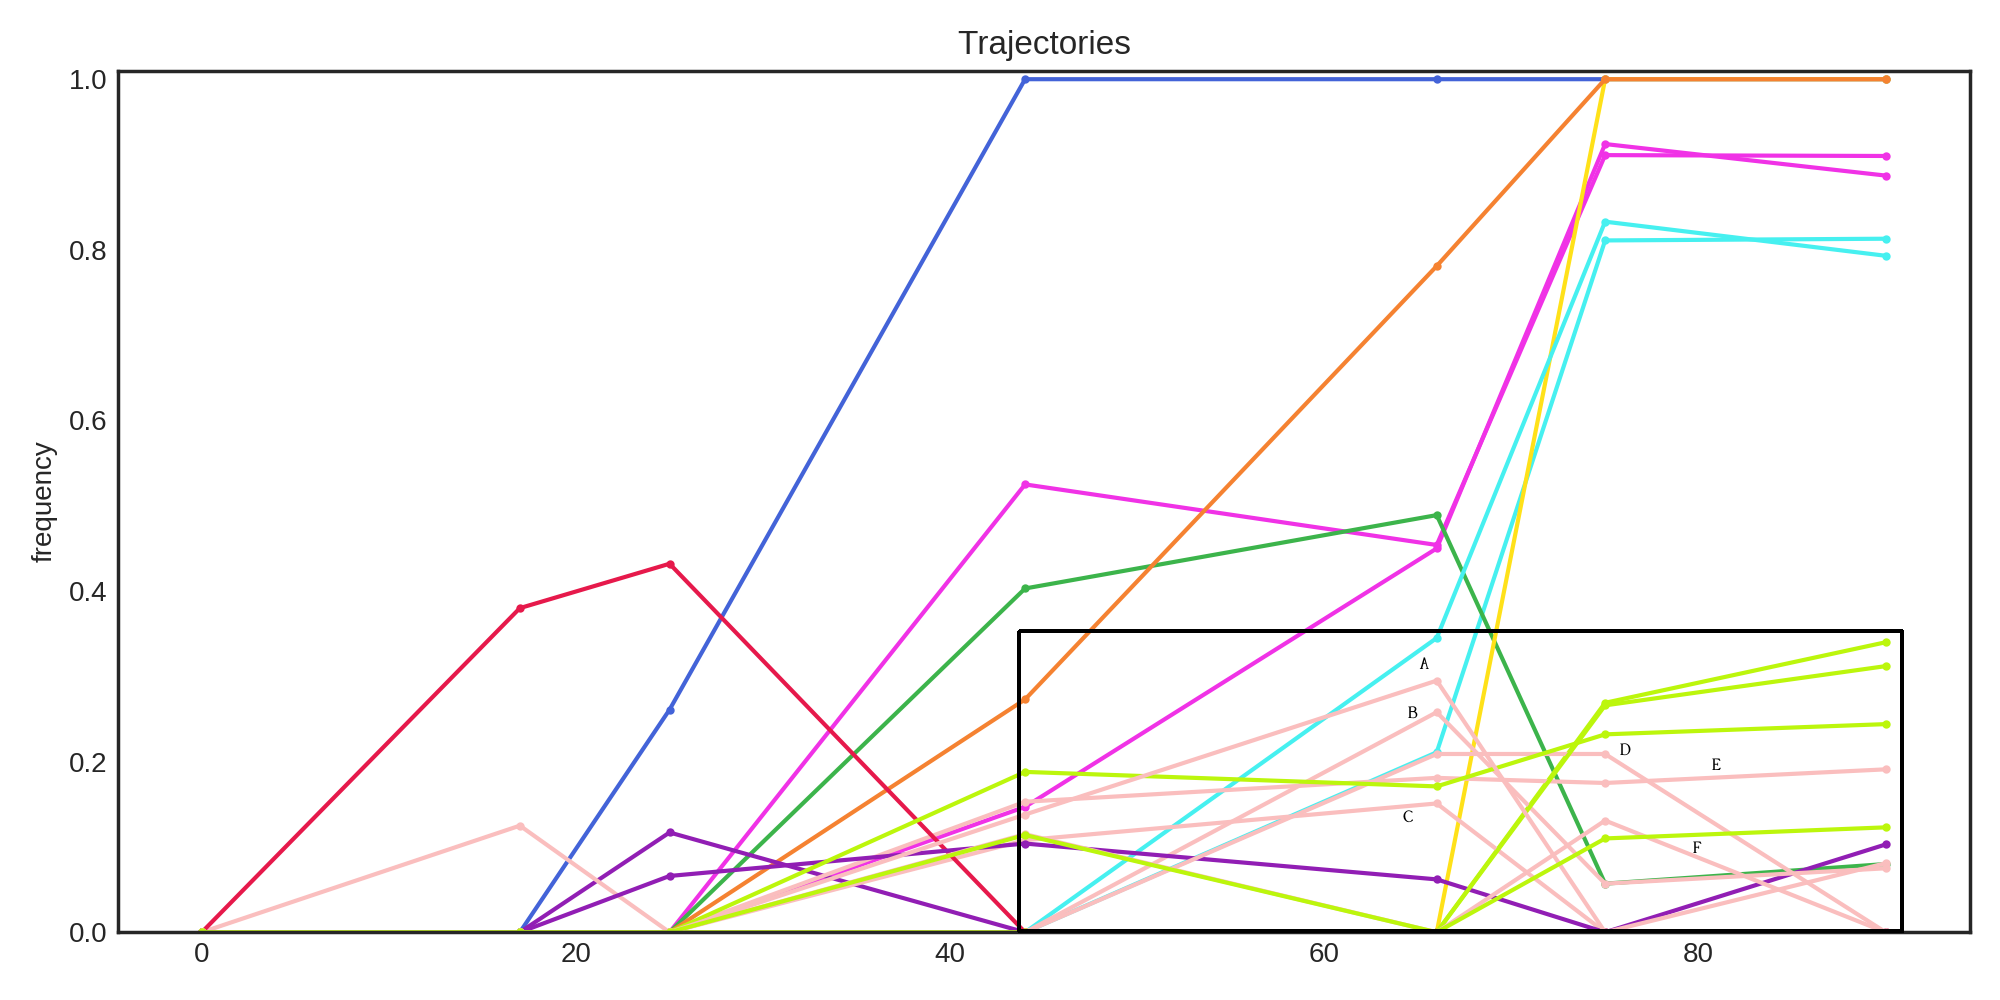
\includegraphics[width=0.5\textwidth]{B1_twostep_trajectories}
\end{figure}
Each line is a single trajectory and is grouped with those of the same color. A major weakness of the two-step clustering method is its inability to accurately extract genotypes during timepoints when a large number of mutational trajectories are detected at similar frequencies. An example of this has been highlighted in the image above, where there are ten trajectories split among three genotypes.

Let's use the tan genotype (consisting of 6 trajectories) as an example. The trajectories labelled A, B, and C appear to be more correlated to each other than to the other three trajectories that have been grouped into this genotype. While the two-step method determined that there was insufficient evidence to group the trajectories into a separate genotype, a human observer may disagree.

Combining the dinomial distance metric with hierarchical clustering provides the following plot:
![B1.hierarchy.binomial.trajectories](figures/B1.hierarchy.binomial.trajectories.png)

This method splits the previous genotype up and groups A and B together (blue), while C (yellow) is paired with another trajectory which was not part of the original genotype, but shares a similar path as C.
\end{document}
